\section{Setpoint Managers }\label{setpoint-managers}

\subsection{Overview}\label{overview-024}

Setpoint Managers are one of the high-level control constructs in EnergyPlus. A Setpoint Manager is able to access data from any of the HVAC system nodes and use this data to calculate a setpoint (usually a temperature setpoint) for one or more other HVAC system nodes. Setpoints are then used by Controllers as a goal for their control actions.

Setpoint managers are executed at the start of each HVAC time step, and they reside outside the HVAC system iteration loops. Thus, the Setpoint Managers are executed once per HVAC time step, and they use previous time step information (except for zone load) to calculate their setpoints.

All temperatures in the following descriptions are in degrees C, loads are in Watts, mass flow rates are in kg/s.

\subsection{Scheduled}\label{scheduled}

The input object SetpointManager:Scheduled provides the simplest setpoint manager that allows the user to specify a seasonal (or other) scheduled reset, for example, of the supply air temperature setpoint.

\begin{equation}
{T_{set}} = {T_{sched}}
\end{equation}

where \({T_{set}}\) is the supply air temperature setpoint and \({T_{sched}}\) is the current value (°C) from the user input temperature schedule. In this case, \({T_{set}}\) will be applied to the node or nodes specified in the input object SetpointManager:Scheduled.~ There are a number of other types of setpoints that can be set, by choosing different control variables in the object, including:

1)~~~Maximum temperature of fluid at node (°C)

2)~~~Minimum temperature of fluid at node (°C)

3)~~~Humidity ratio of fluid at node (kg water/ kg dry air)

4)~~~Maximum humidity ratio of fluid at node (kg water/ kg dry air)

5)~~~Minimum humidity ratio of fluid at node (kg water/ kg dry air)

6)~~~Mass flow rate of fluid at node (kg/s)

7)~~~Maximum mass flow rate of fluid at node (kg/s)

8)~~~Minimum mass flow rate of fluid at node (kg/s)

\subsection{Outdoor Air Reset}\label{outdoor-air-reset}

The input object SetpointManager:OutdoorAirReset provides a setpoint manager that implements an outdoor air reset strategy for the supply air temperature. The user defines a reset rule for this strategy by specifying two setpoint temperatures at two outside drybulb temperatures. Generally the lower setpoint temperature is matched with the higher drybulb temperature and the higher setpoint temperature with the lower drybulb temperature. The user can specify two reset rules and schedule their usage. A schedule value of 1 indicates use of the 1st rule; 2 indicates use of the 2nd.

IF \emph{SchedVal = 2}

\begin{equation}
{T_{out,low}} = {T_{2,out,low}}
\end{equation}

\begin{equation}
{T_{out,high}} = {T_{2,out,high}}
\end{equation}

\begin{equation}
{T_{set,atOAlow}} = {T_{2,set,atOAlow}}
\end{equation}

\begin{equation}
{T_{set,atOAhigh}} = {T_{2,set,atOAhigh}}
\end{equation}

otherwise

\begin{equation}
{T_{out,low}} = {T_{1,out,low}}
\end{equation}

\begin{equation}
{T_{out,high}} = {T_{1,out,high}}
\end{equation}

\begin{equation}
{T_{set,atOAlow}} = {T_{1,set,atOAlow}}
\end{equation}

\({T_{set,atOAhigh}} = {T_{1,set,atOAhigh}}\) .

If \({T_{out,low}} < {T_{out,high}}\) and \({T_{set,atOAlow}} > {T_{set,atOAhigh}}\) ~then

~~~~~ If \({T_{out}} \le {T_{out,low}}\) ~then

~~~~~ \({T_{set}} = {T_{out,low}}\)

~~~~~ if \({T_{out}} \ge {T_{out,high}}\) ~then

~~~~~ \({T_{set}} = {T_{out,high}}\)

~~~~~ otherwise

~~~~~ \({T_{set}} = {T_{set,atOAlow}} - (({T_{out}} - {T_{out,low}})/({T_{out,high}} - {T_{out,low}}))\cdot ({T_{set,atOAlow}} - {T_{set,atOAhigh}})\)

otherwise

~~~~~ \({T_{set}} = 0.5({T_{set,atOAlow}} + {T_{set,atOAhigh)}}\) .

\emph{\({T_{set}}\)}will be applied to the node or nodes specified in the \emph{SetpointManager:OutdoorAirReset} object input.

\subsection{Single Zone Reheat Heating and Cooling}\label{single-zone-reheat-heating-and-cooling}

The input object SetpointManager:SingleZone:Reheat provides a setpoint manager that is used to implement a variable supply air setpoint temperature in which the setpoint is varied~ each timestep to meet the heating or cooling load in a control zone. The manager operates in the following manner.

\begin{equation}
{T_{set}} = {T_z} + {\dot Q_z}/({C_{p,air}}\cdot {\dot m_z})
\end{equation}

where \({T_z}\) is the control zone temperature, \({\dot Q_z}\) is the zone load (greater than zero for heating, less than zero for cooling), \({\dot m_z}\) is the zone supply air mass flow rate, and \({C_{p,air}}\) is the specific heat of air. If \({\dot m_z}\) is very small (\(\le .001\) ~kg/s) \({T_{set}}\) ~is set equal to \({T_{set,min}}\) ~if the control zone has a cooling load and to \({T_{set,max}}\) if the control zone has a heating load. \({T_{set,min}}\) ~is the user specified minimum setpoint and \({T_{set,max}}\) ~is the user specified maximum setpoint. \({T_{set}}\) will be applied to the node or nodes specified in the SetpointManager:SingleZone:Reheat object input.

\subsection{Single Zone Heating Only}\label{single-zone-heating-only}

The input object SetpointManager:SingleZone:Heating provides a model that detects the control zone load to meet the current heating setpoint (Report Variable ``Zone Predicted Sensible Load to Heating Setpoint Heat Transfer Rate {[}W{]}'', zone inlet node flow rate, and zone node temperature, and calculates a setpoint temperature for the supply air that will satisfy the zone heating load for the control zone.~ ``Zone Predicted Sensible Load to Heating Setpoint Heat Transfer Rate {[}W{]}'' \textgreater{} 0 indicates a heating load.~ The following rules are applied:

·~~~~~~~~If there is no zone heating load, then the setpoint is set at the specified minimum supply air temperature.

·~~~~~~~~If there is a zone heating load~ and the zone supply mass flow rate is less than 0.001 kg/s, then the setpoint is set at the specified maximum supply air temperature.

·~~~~~~~~If there is a zone heating load~ and the zone supply mass flow rate is greater than 0.001 kg/s, then the setpoint is set calculated as follows:

\emph{SetPoint = ZoneTemp + ZoneLoadtoHeatSP/(CpAir*ZoneMassFlow)}

where:

\emph{SetPoint =} Setpoint temperature applied to the specified setpoint node(s)

\emph{ZoneTemp =} Current zone temperature

\emph{ZoneLoadtoHeatSP =} Zone heating load (Report Variable " Zone Predicted Sensible Load to Heating Setpoint Heat Transfer Rate {[}W{]}``)

\emph{CpAir =} Specific heat of zone supply air

\emph{ZoneMassFlow =} Zone supply air mass flow rate

\subsection{Single Zone Cooling Only}\label{single-zone-cooling-only}

The input object SetpointManager:SingleZone:Cooling provides a model that detects the control zone load to meet the current cooling setpoint (Report Variable ``Zone Predicted Sensible Load to Cooling Setpoint Heat Transfer Rate {[}W{]}'', zone inlet node flow rate, and zone node temperature, and calculates a setpoint temperature for the supply air that will satisfy the zone cooling load for the control zone.~ ``Zone Predicted Sensible Load to Cooling Setpoint Heat Transfer Rate {[}W{]}'' \textless{} 0 indicates a cooling load.~ The following rules are applied:

·~~~~~~~~If there is no zone cooling load, then the setpoint is set at the specified maximum supply air temperature.

·~~~~~~~~If there is a zone cooling load~ and the zone supply mass flow rate is less than 0.001 kg/s, then the setpoint is set at the specified minimum supply air temperature.

·~~~~~~~~If there is a zone cooling load~ and the zone supply mass flow rate is greater than 0.001 kg/s, then the setpoint is set calculated as follows:

\emph{SetPoint = ZoneTemp + ZoneLoadtoCoolSP/(CpAir*ZoneMassFlow)}

where:

\emph{SetPoint} = Setpoint temperature applied to the specified setpoint node(s)

\emph{ZoneTemp} = Current zone temeprature

\emph{ZoneLoadtoCoolSP} = Zone cooling load (Report Variable ``Zone Predicted Sensible Load to Cooling Setpoint Heat Transfer Rate {[}W{]}'')

\emph{CpAir} = Specific heat of zone supply air

\emph{ZoneMassFlow} = Zone supply air mass flow rate

\subsection{Single Zone Minimum Humidity}\label{single-zone-minimum-humidity}

The input object SetpointManager:SingleZone:Humidity:Minimum provides a model where the zone moisture load from ZoneTempPredictorCorrector (via DataZoneEnergyDemands) is used to calculate the minimum/maximum supply air humidity ratio needed to meet minimum/maximum zone relative humidity requirement.~ For the Max setpoint manager is currently used in Controller:WaterCoil, when the control variable ``TemperatureAndHumidityRatio''.~ A negative MoistureLoad means a dehumidification load for the coil controller.~ This could be used for any system.

\subsection{Single Zone Maximum Humidity}\label{single-zone-maximum-humidity}

The input object SetpointManager:SingleZone:Humidity:Maximum provides a setpoint manager that allows the control of high air humidity levels in a single zone. This setpoint manager, used in conjunction with object ZoneControl:Humidistat, detects the air humidity level in a single control zone and uses air/moisture mass balances to calculate the supply air humidity ratio needed to maintain the zone relative humidity at or below a given setpoint. The calculated supply air humidity ratio is then entered as a setpoint on a designated supply air stream node. A dehumidification component placed upstream of this node can then use the humidity ratio setpoint to control its moisture removal rate (e.g.~desiccant dehumidifiers). In the case of a chilled water coil which is used for both temperature and high humidity control, this setpoint manager works in conjunction with a Controller:WaterCoil object to determine the minimum supply air temperature required to meet both the temperature (sensible) and humidity (latent) load in the control zone. (Ref: Controller:WaterCoil).

\subsubsection{Model Description}\label{model-description-014}

The user must input the required information according to the IO Reference Manual (ref: SetpointManager:SingleZone:Humidity:Maximum). Specific inputs include an object name, control variable (HumidityRatio), name of the schedule defining the maximum relative humidity for the control zone, setpoint node name or list, and the zone air node name associated with the control zone (ref: ZoneHVAC:EquipmentConnections). The schedule name must refer to a valid schedule type (range 0-1) and contain values of fractional relative humidity.

This setpoint manager first converts the desired relative humidity setpoint for the control zone to humidity ratio based on the control zone dry-bulb temperature, the scheduled maximum relative humidity setpoint and outdoor barometric pressure.

\begin{equation}
{\omega_{sp}} = \,{\rm{PsyWFnTdbRhPb}}\left( {{T_{db}},R{H_{sp}},P} \right)
\end{equation}

where:

\({\omega_{sp}}\) ~ = humidity ratio setpoint, kg H\(_{2}\)O/kg air

PsyWFnTdbRHPb = EnergyPlus psychrometric function, returns humidity ratio as a function of dry-bulb temperature, relative humidity, and barometric pressure

\({T_{db}}\) = dry-bulb temperature in the control zone, °C

\(R{H_{sp}}\) = maximum relative humidity setpoint, fraction

\(P\) ~ = outdoor barometric pressure, Pa

The model then calculates the supply air humidity ratio required to reduce the control zone relative humidity to the desired level. Using the humidity ratio setpoint (\({\omega_{sp}}\) ) calculated above,

\begin{equation}
{\omega_{sa}} = \,{\omega_{sp}} + \frac{{{{\mathop Q\limits^ \bullet  }_l}}}{{\mathop m\limits^ \bullet  }}
\end{equation}

where:

\({\omega_{sa}}\) ~ = maximum supply air humidity ratio setpoint, kg H\(_{2}\)O/kg air

\(\mathop {{Q_l}}\limits^ \bullet\) ~ = control zone latent load, kg H\(_{2}\)O/s (calculated by Zone Control:Humidistat)

\(\mathop m\limits^ \bullet\) ~ = control zone mass flow rate, kg/s

All setpoint managers are executed at the beginning of the simulation time step. Therefore, the calculated setpoint is based on the resulting control zone air temperature and air mass flow rate for the previous simulation time step.

The maximum supply air humidity ratio setpoint is placed on the node(s) specified in the input for this object (using node property Humidity Ratio Maximum).

\subsection{Mixed Air}\label{mixed-air}

The input object SetpointManager:MixedAir provides a setpoint manager that takes an already established setpoint (usually the supply air outlet node setpoint temperature), subtracts the supply fan heat gain, and applies the result as the setpoint temperature at the mixed air node (or any other node the user specifies).

\begin{equation}
{T_{set}} = {T_{set,ref}} - ({T_{fan,outlet}} - {T_{fan,inlet}})
\end{equation}

When inputs of optional fields, Cooling Coil Inlet Node Name, Cooling coil Outlet Node Name, and Minimum Temperature at Cooling Coil Outlet Node, are provided, the setpoint temperature at the mixed air node is given below based on supply fan placement and reference node location:

Blow through placement:

\begin{equation}
{T_{set}} = max(T_{set,ref}, T_{min}) - ({T_{coil,outlet}} - {T_{coil,inlet}}) - ({T_{fan,outlet}} - {T_{fan,inlet}})
\end{equation}

Draw through placement:

When the reference node is the cooling coil outlet node:

\begin{equation}
{T_{set}} = max(T_{set,ref}, T_{min}) - ({T_{coil,outlet}} - {T_{coil,inlet}})
\end{equation}

When the reference node is the unitary system outlet node:

\begin{equation}
{T_{set}} = max(T_{set,ref} - ({T_{fan,outlet}} - {T_{fan,inlet}}), T_{min}) - ({T_{coil,outlet}} - {T_{coil,inlet}})
\end{equation}

\subsection{Outdoor Air Pretreat}\label{outdoor-air-pretreat}

The input object SetpointManager:OutdoorAirPretreat provides a setpoint manager that is meant to be used in conjunction with an OutdoorAir:Mixer. The outdoor air pretreat setpoint manager is used to establish a temperature or humidity ratio setpoint in the outdoor air stream flowing into the outdoor air stream node of an outdoor air mixer. This setpoint manager determines the required setpoint in the outdoor air stream to produce the reference setpoint in the mixed air stream after mixing with return air. For example, if the temperature setpoint at the mixed air node is 15C, the return air temperature is 20C, and the outdoor air flow fraction is 0.5, the outdoor air pretreat setpoint would be set to 10C. This setpoint manager references four user-specified nodes to obtain the following values:

·~~~~~~~~Reference setpoint node -- desired mixed flow condition = RefNodeSetPoint

·~~~~~~~~Mixed air stream node -- mixed air flow rate = MixedOutNodeMassFlowRate

·~~~~~~~~Outdoor air stream node -- outdoor air flow rate = OAInNodeMassFlowRate

·~~~~~~~~Return air stream node -- return air condition = ReturnInValue

The following calculations are used to determine the new setpoint value (SetPoint):

\emph{OAFraction = OAInNodeMassFlowRate / MixedOutNodeMassFlowRate}

\emph{SetPoint = ReturnInValue + (RefNodeSetPoint - ReturnInValue)/OAFraction}

Depending on the specified control variable type, the setpoints and conditions may be humidity ratio (max or min) or temperature.~ Note that zero is not allowed as the computed setpoint humidity ratio, because zero is used as a special value to indicate that no humidification or dehumidification is needed.~ If the reference humidity ratio setpoint value is zero, the zero value will be passed directly to the setpoint Node(s).

\subsection{Warmest Zone Supply Air Reset}\label{warmest-zone-supply-air-reset}

The input object SetpointManager:Warmest provides a setpoint manager that attempts to establish a supply air setpoint that will meet the cooling load of the zone needing the coldest air at the maximum zone supply air flowrate. The algorithm loops over all the zones that the system can cool and calculates

\begin{equation}
{T_{set,z}} = {T_z} + {\dot Q_z}/({C_{p,air}}\cdot {\dot m_{z,max}})
\end{equation}

Note that for cooling \({\dot Q_z} < 0.\) The lowest \({T_{set,z}}\) is chosen as \({T_{set}}\) . \({T_{set}}\) is constrained to be less than or equal to the maximum setpoint temperature (user input) and greater than or equal to the minimum setpoint temperature (user input). If the sum of the zone cooling loads is very small, the setpoint temperature is set to the maximum. \({T_{set}}\) will be applied to the node or nodes specified in the SetpointManager:Warmest object input.

\subsection{Coldest Zone Supply Air Reset}\label{coldest-zone-supply-air-reset}

The input object SetpointManager:Coldest provides a setpoint manager that attempts to establish a supply air setpoint that will meet the heating load of the zone needing the warmest air at the maximum zone supply air flowrate. The algorithm loops over all the zones that the system can heat and calculates

\begin{equation}
{T_{set,z}} = {T_z} + {\dot Q_z}/({C_{p,air}}\cdot {\dot m_{z,max}})
\end{equation}

Note that for heating \({\dot Q_z} > 0.\) The highest \({T_{set,z}}\) is chosen as \({T_{set}}\) . \({T_{set}}\) is constrained to be less than or equal to the maximum setpoint temperature (user input) and greater than or equal to the minimum setpoint temperature (user input). If the sum of the zone heating loads is very small, the setpoint temperature is set to the minimum. \({T_{set}}\) will be applied to the node or nodes specified in the SetpointManager:Coldest object input.

\subsection{Return Air Bypass Flow}\label{return-air-bypass-flow}

The input object SetpointManager:ReturnAirBypassFlow provides a setpoint manager that sets the air flow rate in a bypass duct such that when the bypassed and non-bypassed air are mixed the resutant air stream will be at the user-specified setpoint temperature.

The user specifies the desired setpoint temperature \emph{T\(_{set}\)} through a input temperature schedule.

This temperature is modified to account for any potential fan heat gain:

\begin{equation}
{T_{set,mod}} = {T_{set}} - ({T_{loop,out}} - {T_{mixer,out}})
\end{equation}

Here \({T_{loop,out}}\) is the temperature at the air loop outlet node and \({T_{mixer,out}}\) ~is the temperature at the outlet node of the bypass -- nonbypass air mixer. Depending on the system configuration these may be the same node. Then

\begin{equation}
{\dot m_{bypass}} = ({\dot m_{tot}}\cdot {T_{set,mod}} - {\dot m_{nonbypass}}\cdot {T_{nonbypass}})/{T_{bypass}}
\end{equation}

where \({\dot m_{tot}}\) is the total supply air flowrate in kg/s sent to the zones, \({\dot m_{nonbypass}}\) is the nonbypassed air flowrate (the conditioned air), \({T_{nonbypass}}\) is the corresponding temperature just before mixing with the bypassed air, and \({T_{bypass}}\) is the temperature of the bypassed (unconditioned) air. The resulting \({\dot m_{bypass}}\) ~is the mass flow rate setpoint for the bypass air branch.

\subsection{Warmest Temp Flow}\label{warmest-temp-flow}

The input object SetpointManager:WarmestTemperatureFlow provides a setpoint manager that attempts to establish a supply air setpoint that will meet the cooling load of the zone needing the coldest air at the maximum zone supply air flowrate. The supply air temperature setpoint is established by SetpointManager:WarmestTemperatureFlow using one of two strategies: `Temp First' sets the supply air temperature to the highest temperature that will meet the cooling load of the coolest zone at minimum cfm. `Flow First' sets the supply air temperature to the highest temperature that will meet the cooling load of the warmest zone at maximum cfm.~ `Temp First' gives higher priority to reducing fan energy whereas `Flow First' gives higher priority to reducing chiller energy.

The algorithm loops over all the zones that the system can cool and calculates according to strategy:

\textbf{Temp First:}

\begin{equation}
  T_{set,z} = T_z + \frac{\dot{Q}_z}{C_{p,air} \dot{m}_{z,min}}
\end{equation}

\textbf{Flow First:}

\begin{equation}
  T_{set,z} = T_z + \frac{\dot{Q}_z}{C_{p,air} \dot{m}_{z,max}}
\end{equation}

where \({\dot m_{z,\min }}\) is the minimum air flow rate to the zone produced by reducing the capacity of the supply fan or by reducing the opening of the damper in the terminal box, if present, and~ \({\dot m_{z,\max }}\) ~is the design air flow rate to the zone.

Note that for cooling \({\dot Q_z} < 0.\) ~The lowest \({T_{set,z}}\) is chosen as \({T_{set}}\) . \({T_{set}}\) is constrained to be less than or equal to the maximum setpoint temperature (user input) and greater than or equal to the minimum setpoint temperature (user input). If the unconstrained value of \({T_{set}}\) is less than the minimum setpoint temperature and there are no VAV terminal boxes, the fan capacity is increased so as to meet the zone cooling loads with the constrained value of \({T_{set}}\) :

\begin{equation}
{\dot m_{fan}} = \sum\limits_z {{{\dot m}_{z,\min }}}  = \sum\limits_z {{{\dot Q}_z}/[{C_{p,air}} \cdot ({T_{set}} - {T_z})]}
\end{equation}

~This is more likely to occur in the `Temp First' case. If the sum of the zone cooling loads is very small, the setpoint temperature is set to the maximum. \({T_{set}}\) will be applied to the node or nodes specified in the SetpointManager:WarmestTemperatureFlow object input.

\subsection{Multizone Heating Average}\label{multizone-heating-average}

The input object SetpointManager:MultiZone:Heating:Average provides a setpoint manager that attempts to establish a supply air heating setpoint that will meet the heating load of multiple zones served by an HVAC air loop. The algorithm aggregates the predicted heating loads for all controlled zones served by an air loop (i.e., zones that have a thermostat object), and calculates the multizone average supply air heating setpoint temperature as follows:

IF ( \({\dot Q_{zj}}\) \textgreater{} 0 ) THEN

\begin{equation}
\overline {{T_{SP}}}  = \overline {{T_Z}}  + \left( {\frac{{\sum\limits_{j = 1}^{NumControlZones} {{{\dot Q}_{Zi}}} }}{{\sum\limits_{j = 1}^{NumControlZones} {{{\dot m}_{Zi}}\cdot C{p_j}} }}} \right)
\end{equation}

END IF

\begin{equation}
{\bar T_z} = {{\left( {\sum\limits_{j = 1}^{TotZones} {{{\dot m}_{zj}} \bullet } C{p_j} \bullet {T_{zj}}} \right)} \mathord{\left/ {\vphantom {{\left( {\sum\limits_{j = 1}^{TotZones} {{{\dot m}_{zj}} \bullet } C{p_j} \bullet {T_{zj}}} \right)} {\left( {\sum\limits_{j = 1}^{TotZones} {{{\dot m}_{zj}} \bullet } C{p_j}} \right)}}} \right. } {\left( {\sum\limits_{j = 1}^{TotZones} {{{\dot m}_{zj}} \bullet } C{p_j}} \right)}}
\end{equation}

where,

\({\bar T_{SP}}\) ~~~~~~~~~~~~~~~~~ = average supply air setpoint temperature (°C)

\(NumControlZones\) = number of controlled zones (i.e., zones that contain thermostat objects) served by the air loop (-)

\({\dot Q_{Zj}}\) = sensible heating load required to reach the zone air temperature setpoint for the \emph{j}\(^{th}\) controlled zone at current time step (W)

\({\dot m_{Zj}}\) = air mass flow rate being supplied by the air loop to the \emph{j}\(^{th}\) controlled zone, lagged by one HVAC simulation time step (kg/s)

\(C{p_j}\) = specific heat of supply air for the j\(^{th}\) controlled zone (J/kg-K)

\({T_{Zj}}\) = air node temperature for the \emph{j}\(^{th}\) controlled zone (°C)

\({\overline T_Z}\) = average zone air node temperature weighted by the heat capacity rate of the supply air streams for the controlled zones served by the air loop (°C)

\(TotZones\) = total number of zones served by the air loop (-)

Note that for heating \({\dot Q_{Zj}} > 0.\) ~The average supply air setpoint temperature \({\bar T_{SP}}\) ~is constrained to be less than or equal to the maximum setpoint temperature (user input) and greater than or equal to the minimum setpoint temperature (user input). If the sum of the zone sensible heating loads is extremely small (i.e., no heating load), the setpoint temperature is set to the minimum. \({\bar T_{SP}}\) will be applied to the setpoint node or nodes specified in the SetpointManager:MultiZone:Heating:Average object.

\subsection{Multizone Cooling Average}\label{multizone-cooling-average}

The input object SetpointManager:MultiZone:Cooling:Average provides a setpoint manager that attempts to establish a supply air cooling setpoint that will meet the cooling load of multiple zones served by an HVAC air loop. The algorithm aggregates the predicted cooling loads for all controlled zones served by an air loop (i.e., zones that have a thermostat object), and calculates the multizone average supply air cooling setpoint temperature as follows:

IF ( \({\dot Q_{zj}}\) \textless{} 0 ) THEN

\begin{equation}
\overline {{T_{SP}}}  = \overline {{T_Z}}  + \left( {\frac{{\sum\limits_{j = 1}^{NumControlZones} {{{\dot Q}_{Zi}}} }}{{\sum\limits_{j = 1}^{NumControlZones} {{{\dot m}_{Zi}}\cdot C{p_j}} }}} \right)
\end{equation}

END IF

\begin{equation}
{\bar T_z} = {{\left( {\sum\limits_{j = 1}^{TotZones} {{{\dot m}_{Zj}} \bullet } C{p_j} \bullet {T_{zj}}} \right)} \mathord{\left/ {\vphantom {{\left( {\sum\limits_{j = 1}^{TotZones} {{{\dot m}_{Zj}} \bullet } C{p_j} \bullet {T_{zj}}} \right)} {\left( {\sum\limits_{j = 1}^{TotZones} {{{\dot m}_{Zj}} \bullet } C{p_j}} \right)}}} \right. } {\left( {\sum\limits_{j = 1}^{TotZones} {{{\dot m}_{Zj}} \bullet } C{p_j}} \right)}}
\end{equation}

Note that for cooling \({\dot Q_{Zj}} < 0.\) The average supply air setpoint temperature \({\bar T_{SP}}\) is constrained to be less than or equal to the maximum setpoint temperature (user input) and greater than or equal to the minimum setpoint temperature (user input). If the sum of the zone sensible cooling loads is extremely small (i.e., no cooling load), the setpoint temperature is set to the maximum. \({\bar T_{SP}}\) will be applied to the setpoint node or nodes specified in the SetpointManager:MultiZone:Cooling:Average object.

\subsection{Multizone Minimum Humidity Average}\label{multizone-minimum-humidity-average}

The input object SetpointManager:MultiZone:MinimumHumidity:Average provides a setpoint manager that attempts to establish a supply air minimum humidity ratio setpoint that will meet the humidification load of multiple zones served by an HVAC air loop.~ This setpoint manager, used in conjunction with object ZoneControl:Humidistat, detects the air humidity level for all controlled zones served by an air loop (i.e., zones that have a humidistat object with a humidifying setpoint schedule), and uses moisture mass balances to calculate the average supply air minimum humidity ratio setpoint as follows:

IF ( \({\dot Q_{lzj}}\) \textgreater{} 0 ) THEN

\begin{equation}
  \bar{\omega}_{SP} = \bar{\omega}_Z + \frac{\sum\limits_{j = 1}^{NumControlZones}\dot{Q}_{l,Zj}}{\sum\limits_{j = 1}^{NumControlZones}\dot{m}_{ZJ}}
\end{equation}

END IF

\begin{equation}
  \bar{\omega}_{Z} = \frac{\sum\limits_{j = 1}^{TotZones}\dot{m}_{Zj}\omega_{Zj}}{\sum\limits_{j = 1}^{TotZones}\dot{m}_{ZJ}}
\end{equation}

where,

\({\bar \omega_{SP}}\) = average supply air minimum humidity ratio setpoint (kg H\(_{2}\)O/kg air)

\(NumControlZones\) = number of controlled zones (i.e., zones that contain humidistat objects with humidifying setpoint schedule) served by the air loop (-)

\({\dot Q_{lZj}}\) = latent (humidification) load required to reach the zone air humidifying setpoint for the \emph{j}\(^{th}\) controlled zone at current time step (kg H\(_{2}\)O/s)

\({\dot m_{Zj}}\) = air mass flow rate being supplied by the air loop to the \emph{j}\(^{th}\) controlled zone, lagged by one HVAC simulation time step (kg/s)

\({\omega_{Zj}}\) = air node humidity ratio for the jth controlled zone (kg H\(_{2}\)O/kg air)

\({\bar \omega_Z}\) = average zone air node humidity ratio weighted by supply air mass flow rate for the controlled zones served by the air loop (kg H\(_{2}\)O/kg air)

\(TotZones\) = total number of zones served by the air loop (-)

Note that a positive latent load means humidification is required. The average supply air minimum humidity ratio setpoint \({\bar \omega_{SP}}\) is constrained to be less than or equal to the maximum setpoint humidity ratio (user input) and greater than or equal to the minimum setpoint humidity ratio (user input). If the sum of the zone latent humidification loads is extremely small (i.e., no humidification load), the humidity ratio setpoint is set to the minimum. \({\bar \omega_{SP}}\) will be applied to the setpoint node or nodes specified in the SetpointManager:MultiZone:MinimumHumidity:Average object. A humidification component (e.g., an electric humidifier) placed upstream of this node can then use the humidity ratio setpoint to control its moisture addition rate.

All setpoint managers are executed at the beginning of the simulation time step. Therefore, the calculated setpoint is based on the resulting zone air node humidity ratios and supply air mass flow rates for the previous simulation time step.

\subsection{Multizone Maximum Humidity Average}\label{multizone-maximum-humidity-average}

The input object SetpointManager:MultiZone:MaximumHumidity:Average provides a setpoint manager that attempts to establish a supply air maximum humidity ratio setpoint that will meet the dehumidification load of multiple zones served by an HVAC air loop. This setpoint manager, used in conjunction with object ZoneControl:Humidistat, detects the air humidity level for all controlled zones served by an air loop (i.e., zones that have a humidistat object with a dehumidifying setpoint schedule), and uses moisture mass balances to calculate the average supply air maximum humidity ratio as follows:

IF ( \({\dot Q_{lzj}}\) \textless{} 0 ) THEN

\begin{equation}
  \bar{\omega}_{SP} = \bar{\omega}_Z + \frac{\sum\limits_{j = 1}^{NumControlZones}\dot{Q}_{l,Zj}}{\sum\limits_{j = 1}^{NumControlZones}\dot{m}_{ZJ}}
\end{equation}

END IF

\begin{equation}
  \bar{\omega}_{Z} = \frac{\sum\limits_{j = 1}^{TotZones}\dot{m}_{Zj}\omega_{Zj}}{\sum\limits_{j = 1}^{TotZones}\dot{m}_{ZJ}}
\end{equation}

Note that a negative latent load means dehumidification is required. The average supply air maximum humidity ratio setpoint \({\bar \omega_{SP}}\) is constrained to be less than or equal to the maximum setpoint humidity ratio (user input) and greater than or equal to the minimum setpoint humidity ratio (user input). If the sum of the zone latent dehumidification loads is extremely small (i.e., no dehumidification load), the humidity ratio setpoint is set to the maximum. \({\bar \omega_{SP}}\) will be applied to the setpoint node or nodes specified in the SetpointManager:MultiZone:MaximumHumidity:Average object. A dehumidification component (e.g., an desiccant dehumidifier) placed upstream of this node can then use the humidity ratio setpoint to control its moisture removal rate. In the case of a chilled water coil which is used for both temperature and high humidity control, this setpoint manager works in conjunction with a Controller:WaterCoil object to determines the minimum supply air temperature required to meet both the temperature (sensible) and humidity (latent) load in the control zone (ref: Controller:WaterCoil).

\subsection{MultiZone Minimum Humidity Supply Air Reset}\label{multizone-minimum-humidity-supply-air-reset}

The input object SetpointManager:MultiZone:Humidity:Minimum provides a setpoint manager that attempts to establish a supply air minimum humidity ratio setpoint that will meet the humidification load of zone with the critical humidification requirement at each time step served by an HVAC air loop at the zone actual supply air mass flow rate.~ This setpoint manager, used in conjunction with object ZoneControl:Humidistat, detects the air humidity level for all controlled zones served by an air loop (i.e., zones that have a humidistat object with a humidifying setpoint schedule), and uses moisture mass balances to calculate the supply air minimum humidity ratio setpoint.~ The algorithm loops over all the zones that the system can humidify and calculates the setpoint based on a zone with the highest humidity ratio setpoint requirement as follows:

IF (\({\dot Q_{lzj}}\) \textgreater{} 0) THEN

\begin{equation}
{\omega_{SP\;Zj}} = {\omega_{Zj}} + {{{{\dot Q}_{lZj}}} \mathord{\left/ {\vphantom {{{{\dot Q}_{lZj}}} {{{\dot m}_{Zj}}}}} \right. } {{{\dot m}_{Zj}}}}
\end{equation}

END IF

\begin{equation}
{\omega_{SP\;Zj}} = MAX\left( {{\omega_{SP\;Zj}},\;{\omega_{SP\;Min}}} \right)
\end{equation}

\begin{equation}
{\omega_{SP}} = MIN\left( {{\omega_{SP\;Zj}},\;{\omega_{SP\;Max}}} \right)
\end{equation}

where,

\({\omega_{SP}}\) = supply air humidity ratio setpoint (kg/kg)

\({\dot Q_{lzj}}\) = latent load required to reach the zone air setpoint for the \emph{j}\(^{th}\) controlled zone at current time step (kg H\(_{2}\)O/s)

\({\dot m_{Zj}}\) = actual mass flow rate supplied by the air loop to the \emph{j}\(^{th}\) controlled zone, (kg/s)

\({\omega_{Zj}}\) = air node humidity ratio for the j\(^{th}\) controlled zone (kg/kg)

\({\omega_{SP\;Zj}}\) = supply air humidity ratio setpoint for the j\(^{th}\) controlled zones (kg/kg)

\({\omega_{SP\;Min}}\) = user-specified supply air minimum humidity ratio setpoint (kg/kg)

\({\omega_{SP\;Max}}\) = user-specified supply air maximum humidity ratio setpoint (kg/kg)

Note that a positive latent load means humidification is required. The supply air minimum humidity ratio setpoint \({\omega_{SP}}\) is constrained to be less than or equal to the maximum setpoint humidity ratio (user input) and greater than or equal to the minimum setpoint humidity ratio (user input). If the humidification load for all zones in the air loop is extremely small (i.e., no humidification load), the humidity ratio setpoint is set to the user input minimum value. \({\omega_{SP}}\) will be applied to the setpoint node or nodes specified in the SetpointManager:MultiZone:Humidity:Minimum object. A humidification component (e.g., an electric humidifier) placed upstream of this node can then use the humidity ratio setpoint to control its moisture addition rate.

\subsection{MultiZone Maximum Humidity Supply Air Reset}\label{multizone-maximum-humidity-supply-air-reset}

The input object SetpointManager:MultiZone:Humidity:Maximum provides a setpoint manager that attempts to establish a supply air maximum humidity ratio setpoint that will meet the dehumidification load of the zone with the critical dehumidification requirement at each time step served by an HVAC air loop at the zone actual supply air mass flow rate. This setpoint manager, used in conjunction with object ZoneControl:Humidistat, detects the air humidity level for all controlled zones served by an air loop (i.e., zones that have a humidistat object with a dehumidifying setpoint schedule), and uses moisture mass balances to calculate the supply air maximum humidity ratio setpoint.~ The algorithm loops over all the zones that the system can dehumidify and calculates the setpoint based on a zone with the lowest humidity ratio setpoint requirement as follows:

IF (\({\dot Q_{lzj}}\) \textless{} 0) THEN

\begin{equation}
{\omega_{SP\;Zj}} = {\omega_{Zj}} + {{{{\dot Q}_{lZj}}} \mathord{\left/ {\vphantom {{{{\dot Q}_{lZj}}} {{{\dot m}_{Zj}}}}} \right. } {{{\dot m}_{Zj}}}}
\end{equation}

END IF

\begin{equation}
{\omega_{SP\;Zj}} = MAX\left( {{\omega_{SP\;Zj}},\;{\omega_{SP\;Min}}} \right)
\end{equation}

\begin{equation}
{\omega_{SP}} = MIN\left( {{\omega_{SP\;Zj}},\;{\omega_{SP\;Max}}} \right)
\end{equation}

Note that a negative latent load means dehumidification is required. The supply air maximum humidity ratio setpoint \({\omega_{SP}}\) is constrained to be less than or equal to the maximum setpoint humidity ratio (user input) and greater than or equal to the minimum setpoint humidity ratio (user input). If the dehumidification load for all zones in the air loop is extremely small (i.e., no dehumidification load), the humidity ratio setpoint is set to the user input maximum value. \({\omega_{SP}}\) will be applied to the setpoint node or nodes specified in the SetpointManager:MultiZone:Humidity:Maximum object. A dehumidification component (e.g., an desiccant dehumidifier) placed upstream of this node can then use the humidity ratio setpoint to control its moisture removal rate. In the case of a chilled water coil which is used for both temperature and high humidity control, this setpoint manager works in conjunction with a Controller:WaterCoil object to determines the minimum supply air temperature required to meet both the temperature (sensible) and dehumidification (latent) load in the control zone (ref: Controller:WaterCoil).

\subsection{Follow Outdoor Air Temperature}\label{follow-outdoor-air-temperature}

The input object SetpointManager:FollowOutdoorAirTemperature provides a setpoint manager that is used to place a temperature setpoint on a system node that is derived from the current outdoor air environmental conditions.~ The outdoor air conditions are obtained from the weather information during the simulation.

IF (ReferenceTemperatureType = = OutdoorWetBulb)

~~~ Setpoint = OutdoorWetBulbTemp + OffSet

ELSEIF (ReferenceTemperatureType = = OutdoorDryBulb)

~~~ Setpoint = OutdoorDryBulbTemp + OffSet

ENDIF

Setpoint = MAX(Setpoint, MinSetPoint)

Setpoint = MIN(Setpoint, MaxSetPoint)

MinSetPoint, MaxSetPoint and Offset are specified by the user as the input in object SetpointManager:FollowOutdoorAirTemperature.

\subsection{Follow System Node Temperature}\label{follow-system-node-temperature}

The input object SetpointManager:FollowSystemNodeTemperature provides a temperature setpoint on a system node that is derived from the current temperatures at a separate system node.~ The current value of the temperature at a reference node are obtained and used to generate setpoint on a second system node.~ If the reference node is also designated to be an outdoor air (intake) node, then this setpoint manager can be used to follow outdoor air conditions that are adjusted for altitude.

IF (ReferenceTemperatureType = = NodeWetBulb)

~~~ Setpoint = NodeWetbulbTemp + OffSet

ELSEIF (ReferenceTemperatureType = = NodeDryBulb)

~~~ Setpoint = NodeDrybulbTemp + OffSet

ENDIF

Setpoint = MAX(Setpoint, MinSetPoint)

Setpoint = MIN(Setpoint, MaxSetPoint)

MinSetPoint, MaxSetPoint and Offset are specified by the user as the input in object SetpointManager:FollowSystemNodeTemperature.

\subsection{Follow Ground Temperature}\label{follow-ground-temperature}

The input object SetpointManager:FollowGroundTemperature provides a temperature setpoint on a system node that is derived from a current ground temperature.~ The ground temperatures are specified in different Site:GroundTemperature:* objects and used during the simulation.~ This setpoint manager is primarily intended for condenser or plant loops using some type of ground heat exchanger.

IF (ReferenceGroundTemperatureObjectType = = BuildingSurface)

~~~ Setpoint = GroundTemp + OffSet

ELSEIF (ReferenceGroundTemperatureObjectType = = Shallow)

~~~ Setpoint = GroundTemp\_Surface + OffSet

ELSEIF (ReferenceGroundTemperatureObjectType = = Deep)

~~~ Setpoint = GroundTemp\_Deep + OffSet

ELSEIF (ReferenceTGroundTemperatureObjectType = = FCfactorMethod)

~~~ Setpoint = GroundTemp\_FC + OffSet

ENDIF

Setpoint = MAX(Setpoint, MinSetPoint)

Setpoint = MIN(Setpoint, MaxSetPoint)

\emph{~}

Where,

GroundTemp = Current ground temperature (C)

(Ref: Site:GroundTemperature:BuildingSurface)

GroundTemp\_Surface = Current surface ground temperature~ (C)

(Ref: Site:GroundTemperature:Shallow)

GroundTemp\_Deep~ = Current deep ground temperature~ (C)

(Ref: Site:GroundTemperature:Deep)

GroundTemp\_FC = Current ground temperature defined F or C factor method (C)

(Ref: Site:GroundTemperature:FCfactorMethod)

MinSetPoint, MaxSetPoint and Offset are specified by the user as the input in object SetpointManager:FollowGroundTemperature.

\subsection{Condenser Entering Water Temperature Reset}\label{condenser-entering-water-temperature-reset}

The object resets the condenser entering water temperature to the optimal cooling tower water set point temperature that will result in minimum net energy consumption for the chiller and cooling tower plant. This chiller-tower optimization scheme uses one curve to determine the optimum condenser entering water temperature for a given time step and two other curves to place limit conditions on the ``optimized'' set point value. The optimized condenser entering water temperature may not be valid every timestep then will be limited algorithmically by two boundary curves. The first of these boundary curves is given by:

\emph{MinDsnWB = C1 + C2*OaWb + C3*WPLR + C4*TwrDsnWB + C5*NF}

where:

\emph{C1-C5} = curve coefficients

\emph{OaWb} = outside air wetbulb for current timestep, C

\emph{TwrDsnWB} = Tower design inlet Air Wet-Bulb Temperature, C

\emph{WPLR} = Weighted PLR

~~~ = ChillerCoolingLoadThisTimestep / NominalChillerCapacity

NF = Normalized condenser water flow per unit of tower capacity, m3/W

~~~~~ = Design Tower Flow Rate / Design Tower Capacity \emph{(typically 5.382E-8 m3/s, i.e., 3 gpm/ton)}

MinDsnWB is compared against the design tower wetbulb. This curve is usually a function of Weighted PLR and NF. So if NF is constant at 5.382E-8 m3/s (3 gpm/ton), the curve can be depicted as follows:

\begin{figure}[hbtp] % fig 292
\centering
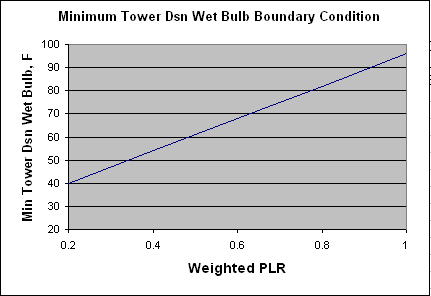
\includegraphics[width=0.9\textwidth, height=0.9\textheight, keepaspectratio=true]{media/image6482.png}
\caption{Minimum Tower Design Wet Bulb Boundary Condition \protect \label{fig:minimum-tower-design-wet-bulb-boundary}}
\end{figure}

The second boundary curve is given by:

\emph{MinActualWb = C1 + C2*MinDsnWB + C3*WPLR + C4*TwrDsnWB + C5*NF}

where,

\emph{C1-C5 = curve coefficients}

\emph{MinDsnWB = from first boundary equation, C}

\emph{TwrDsnWB = Tower design inlet Air Wet-Bulb Temperature, C}

\emph{WPLR = Weighted PLR}

\emph{~~~~~~~~~~ = ChillerCoolingLoadThisTimestep / NominalChillerCapacity}

\emph{NF = Normalized condenser water flow per unit of tower capacity, m3/W}

\emph{~~~~~ = Design Tower Flow Rate / Design Tower Capacity (typically 5.382E-8 m3/s, i.e., 3 gpm/ton)}

MinActualWb is compared against this time step's outside air wet bulb. This curve is usually a function of MinDesignWB, WeightedRatio and TwrDesignWB. So if TwrDesignWB is constant at 25.6 °C (78 °F), and NF = 5.382E-8 m3/s (3 gpm/ton), the curve can be depicted as follows:

\begin{figure}[hbtp] % fig 293
\centering
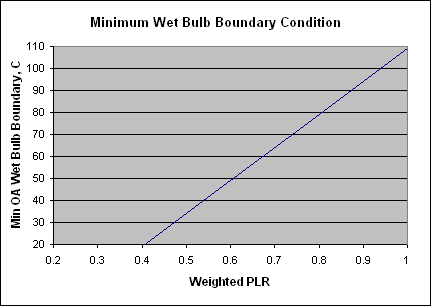
\includegraphics[width=0.9\textwidth, height=0.9\textheight, keepaspectratio=true]{media/image6483.png}
\caption{Minimum Wet Bulb Boundary Condition \protect \label{fig:minimum-wet-bulb-boundary-condition}}
\end{figure}

The Optimized Condenser Entering Water Temperature is calculated with this equation:

\emph{OptCondEntTemp = C1 + C2*OaWb + C3*WPLR + C4*TwrDsnWB + C5*NF}

where,

\emph{C1-C5 = curve coefficients}

\emph{OaWB = this timestep's outside air wetbulb, C}

\emph{TwrDsnWB = Tower design inlet Air Wet-Bulb Temperature, C}

\emph{WPLR = Weighted PLR}

\emph{~~~~~~~~~~ = ChillerCoolingLoadThisTimestep / NominalChillerCapacity}

\emph{NF = Normalized condenser water flow per unit of tower capacity, m3/W}

\emph{~~~~~ = Design Tower Flow Rate / Design Tower Capacity (typically 5.382E-8 m3/s, i.e., 3 gpm/ton)}

A graph of the curve can be depicted as follows:

\begin{figure}[hbtp] % fig 294
\centering
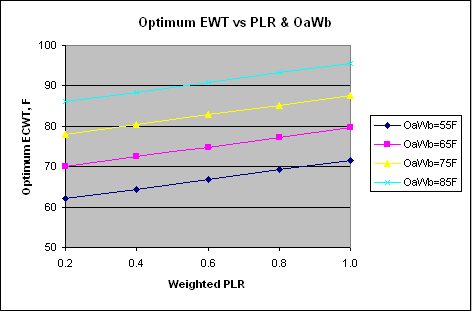
\includegraphics[width=0.9\textwidth, height=0.9\textheight, keepaspectratio=true]{media/image6484.png}
\caption{Optimum EWT vs PLR \& OaWb \protect \label{fig:optimum-ewt-vs-plr-oawb}}
\end{figure}

The optimized condenser entering water temperature is calculated but is not necessarily used each timestep. If OptCondEntTemp does not fall within the bounds established by MinDsnWB and MinActualWb, then the value from the Default Condenser Entering Water Temperature Schedule is used for the Condenser Entering Water Set Point instead.

\subsubsection{Special Note for Multiple Towers}\label{special-note-for-multiple-towers}

This control scheme is available for multiple towers by following two steps:

\begin{itemize}
\tightlist
\item
  Use average tower conditions in the curves for the independent variables related to the towers
\item
  Make sure the setpoint is applied to either the condenser supply outlet node or use a node list to apply it to each tower outlet node
\end{itemize}

\subsection{Ideal Condenser Entering Water Temperature Reset}\label{ideal-condenser-entering-water-temperature-reset}

The object determines a ``near-optimal'' condenser water entering set point at each time step that will result in minimum net energy consumption for the chiller and cooling tower plant. The ``ideal'' chiller-tower optimization scheme uses a search algorithm to find the ideal optimal setpoint at a given timestep. This requires resimulating HVAC systems at each timestep until finding an ``optimal'' condenser water entering setpoint (OptSetpoint) which gives the minimum total chiller, cooling tower, chilled water pump and condenser water pump power consumption (TEC). The OptSetpoint falls between realistic minimum and maximum boundaries, which are set by the user. The minimum boundary is determined based on the minimum lift (user input) and evaporator leaving water temperature. The maximum boundary is specified by the user. It is assumed that a single minimum point exists between these boundaries. The following steps are used to find ``optimal'' setpoint:

1)~~~Set an initial setpoint value for the iteration to a user-defined maximum condenser entering water temperature (Toptset\(_{1}\)) and calculate TEC.

2)~~~Decrease the setpoint value by 1˚C (Toptset\(_{2}\) = Toptset\(_{1}\)--1˚C) and calculate TEC.

3)~~~Compare the TEC in Step 1 (TEC\(_{1}\)) and TEC in Step 2 (TEC\(_{2}\)), i.e., (dTEC\(_{1}\) = TEC\(_{1}\)--TEC\(_{2}\)).

4)~~~If dTEC\(_{1}\) is negative, stop the iteration and set the ``optimal'' setpoint to Toptset\(_{1}\).

5)~~~If dTEC\(_{1}\) is positive, Decrease the setpoint value by 1˚C and calculate TEC. Compare the TECs and repeat this step (i.e., dTEC\(_{N}\) = TEC\(_{N}\)--TEC\(_{N+1}\)) until either Toptset\(_{N+1}\) reaches to the minimum boundary value or dTEC\(_{N}\) becomes negative.

6)~~~If Toptset\(_{N}\) reaches to the minimum boundary value and still dTEC\(_{N}\) is positive, set the ``optimal'' setpoint to Toptset\(_{N+1}\).

7)~~~If TEC\(_{N}\) becomes negative, decrease Toptset\(_{N-1}\) by 0.2˚C and calculate TEC. Compare the TECs and repeat this step (i.e., dTEC\(_{M}\) = TEC\(_{M}\)--TEC\(_{M+1}\)) until dTEC\(_{M}\) becomes negative. Then set the ``optimal'' setpoint to Toptset\(_{M+1}\).

\subsection{Plant Return Water Control Setpoint Reset}\label{plant-return-water-control-setpoint-reset}

The input objects:

\begin{itemize}
\item
  SetpointManager:ReturnTemperature:ChilledWater, and
\item
  SetpointManager:ReturnTemperature:HotWater
\end{itemize}

allow for controlling the temperature of the water (or a different fluid defined for the plant) that is returning back to the plant supply equipment. In a typical chilled water loop configuration, this is essentially controlling the temperature of the water entering the chiller. In a typical hot water loop configuration, this is essentially controlling the temperature of the water entering the boiler.

The target return temperature can be specified by:

\begin{itemize}
\item
  providing a constant value to use throughout the simulation, or
\item
  scheduling the value to vary through the simulation (which then allows custom EMS overriding of the scheduled value), or
\item
  using a separate setpoint manager to set the setpoint on the return node itself, which is then retrieved by this reset manager.
\end{itemize}

\subsubsection{Operation}\label{operation}

The setpoint manager senses conditions on two named nodes, which should correspond to a central plant's supply side inlet and outlet nodes, the return and supply nodes, respectively. The temperature and flow rate information is used in a series of calculations in order to determine a setpoint to specify on the supply outlet node which will in turn provide the target desired return temperature on the supply inlet node. The calculations are summarized for a chilled water loop here:

\begin{enumerate}
\def\labelenumi{\arabic{enumi}.}
\item
  Use the current supply and demand temperatures to calculate an average temperature for property calculation: \(C_p = f\left(T_{avg}\right) = f\left(\frac{T_{ret}+T_{sup}}{2}\right)\)
\item
  Calculate the current loop demand using: \(\dot{Q} = \dot{m} * C_p * \left(T_{ret} - T_{sup}\right)\)
\item
  Assuming that this load will be the same moving forward, we can calculate what supply temperature we should target in order to meet the desired return temperature.
\item
  So retrieve the current target return temperature, \(T_{ret,target}\) , either from a schedule or constant value.
\item
  Then calculate the supply temperature setpoint using: \(T_{sup,sp} = T_{ret,target} - \frac{\dot{Q}}{\dot{m} C_p}\)
\item
  Constrain the value to user-specified limiting min/max values
\end{enumerate}

For a chilled water loop, the user-specified minimum is the default setpoint used in cases of no-load or negative-load. In a hot-water loop the user-specified maximum is used for these situations. Also, in a hot-water loop the sign of the demand will be reversed.

\subsubsection{Key control note}\label{key-control-note}

The setpoint will be reset at the beginning of a system time step, and remain that way through that time step. The setpoint is calculated based on the latest known value of loop demand and loop flow rate. If the demand and flow rate remain the same for the currently calculated time step, the loop will maintain control well. However, if either changes, there will be a lag effect while the loop attempts to maintain control. Consider the following plot, with a short description following:

\begin{figure}[htbp]
\centering
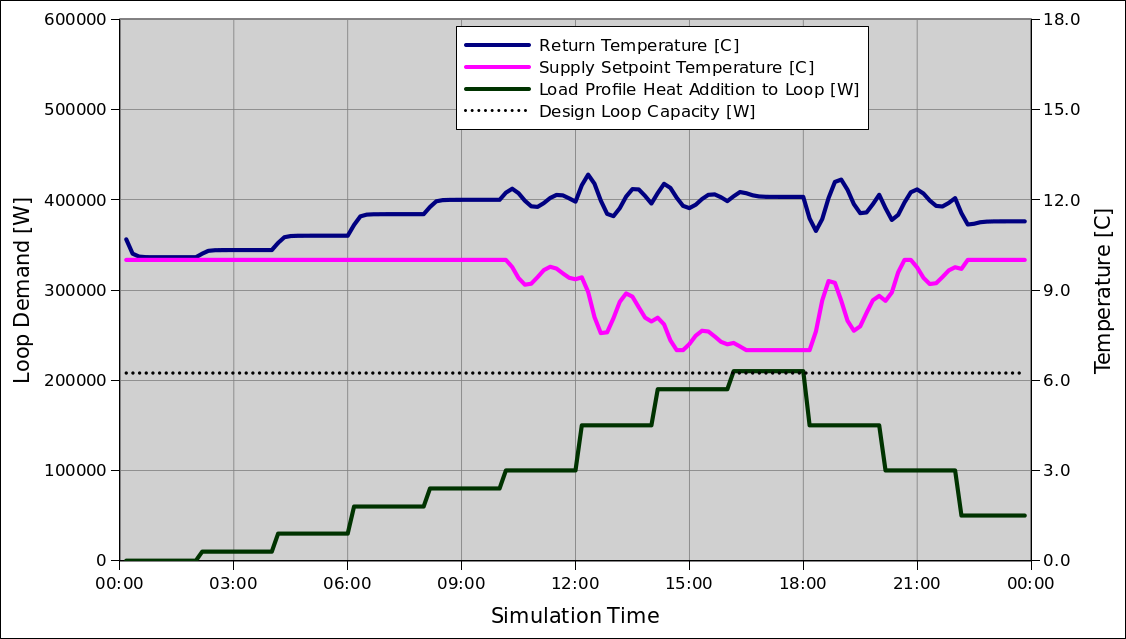
\includegraphics{media/SetPointManager-ResetForReturnControl1.png}
\caption{}
\end{figure}

Throughout the day, the heat addition (green line) to the loop increases. Each time it increases, there is a small period of time where the loop attempts to regain control of the return temperature. The setpoint is only reset at the beginning of the system time step, so as the plant converges within a single time step, the load will vary and the return temperature may not be exactly on target.

This isn't necessarily a big problem. However, some users may be especially interested in very tight control of the return temperature. This can be done very easily by simply reducing the simulation time step. For example, in the following plot, the time step was reduced from 10 minutes to 1 minute, with some description following the plot:

\begin{figure}[htbp]
\centering
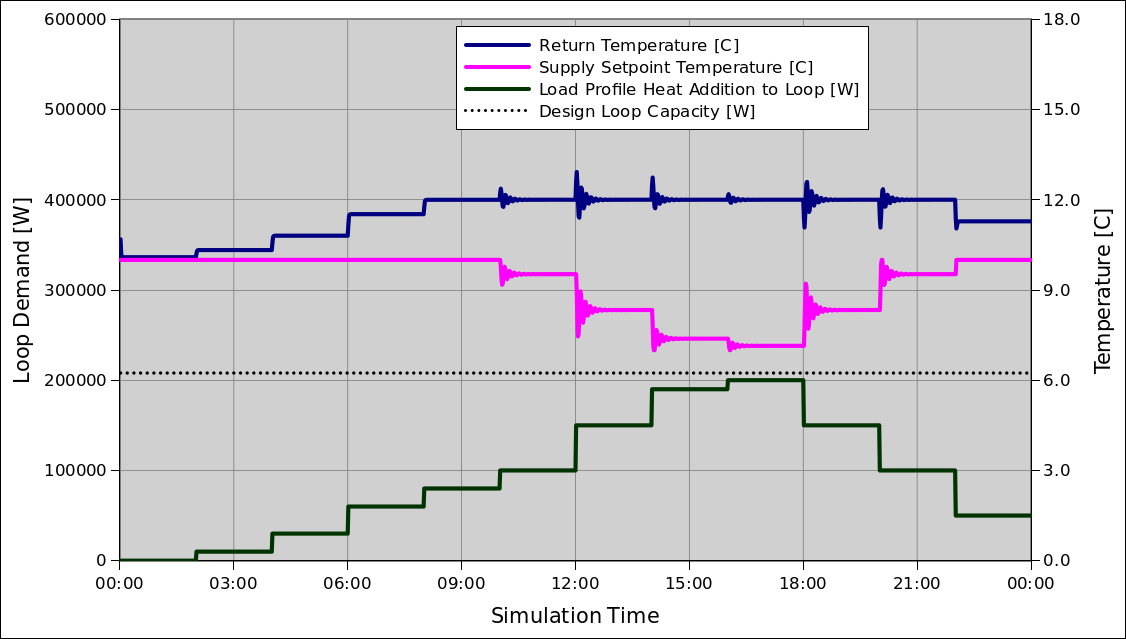
\includegraphics{media/SetPointManager-ResetForReturnControl2.png}
\caption{}
\end{figure}

With the smaller time step, the reporting frequency is higher. But more importantly, with the smaller time step, the setpoint can be corrected much more often. Because of this, the return temperature regains control much quicker than with the larger time step.

However, these examples are for a jagged demand profile full of discontinuous step changes in loop demand. As a final example, this return water temperature control is applied to the large office reference building chilled water loop. Here is the response:

\begin{figure}[htbp]
\centering
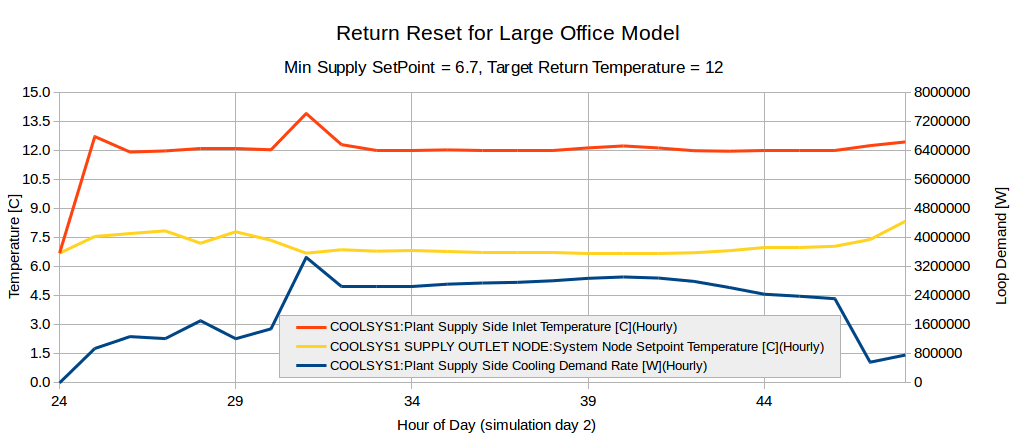
\includegraphics{media/SetPointManager-ResetForReturnControl3.png}
\caption{}
\end{figure}

Note the control is working properly, maintaining a return temperature around the target of 12 degrees where possible. Since the load profile is a typical -smooth- profile, the control is also much smoother. This should be a good representation of the capabilities of this setpoint manager.

For jagged load profiles, if tight control is highly important, choosing a smaller timestep (\textasciitilde{}1 minute) is recommended. For normal building profiles, the typical range of timesteps (\textasciitilde{}15 minute) should be fully satisfactory.
